\setchapterimage{fig_00}

\renewcommand{\titrechapitre}{Tête de découpe de tissus}

\chapter*{TD \arabic{cptTD} \\ 
\titrechapitre -- \ifprof Corrigé \else Sujet \fi}
\addcontentsline{toc}{section}{TD \arabic{cptTD} : \titrechapitre -- \ifprof Corrigé \else Sujet \fi}
\iflivret \stepcounter{cptTD} \else
\ifprof  \stepcounter{cptTD} \else \fi
\fi

\renewcommand{\leftmark}{\titrechapitre}
\renewcommand{\rightmark}{\titrechapitre}


\setcounter{question}{0}

\marginnote{Concours CCINP MP 2018.}
\marginnote{\UPSTIcompetence[2]{B2-07}}
\begin{marginfigure}
\centering
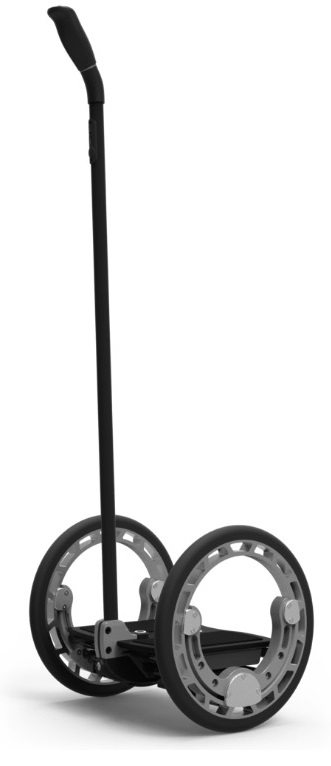
\includegraphics[width=.9\linewidth]{fig_01}
\end{marginfigure}

\ifprof
\else
Un système de découpe automatisé de tissus est composé (figure \ref{cy_01_ch_02_03_td_03_fig_02}):
\begin{itemize}
\item d’une table de découpe sur laquelle le tissus à découper (appelé matelas) est maintenu en position
par aspiration;
\item d’un bras transversal qui se déplace en translation de direction $\vect{y_0}$ par rapport à la table;
\item d’une tête de coupe qui se déplace en translation de direction $\vect{x_0}$ par rapport au bras transversal;
\item d’un ordinateur qui pilote l’ensemble du système.
\end{itemize}


\begin{marginfigure}%[!h]
\centering
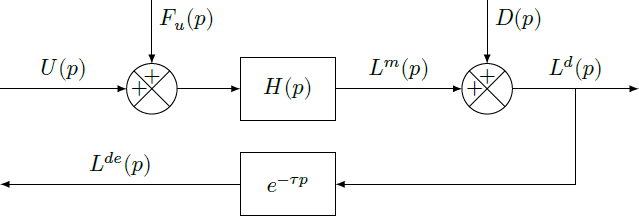
\includegraphics[width=\linewidth]{fig_02}
\caption{Structure d’une table de découpe de tissus}
\label{cy_01_ch_02_03_td_03_fig_02}
\end{marginfigure}

\fi

\begin{marginfigure}
\centering
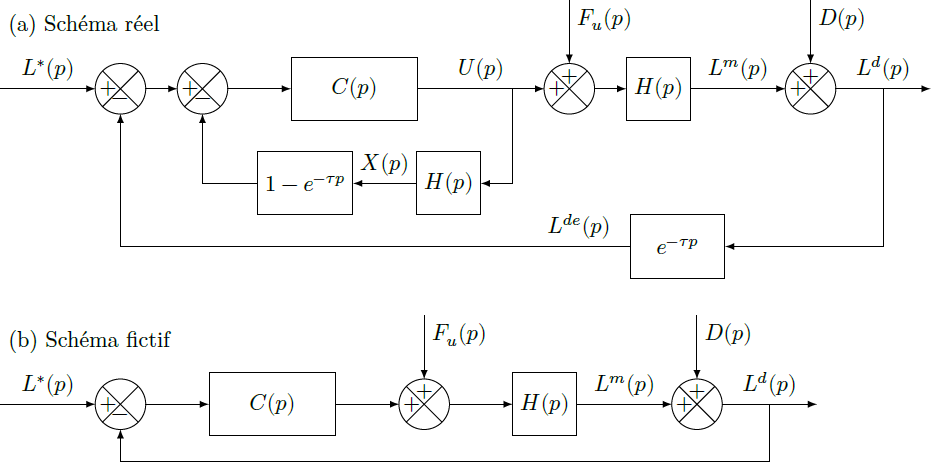
\includegraphics[width=\linewidth]{fig_04}
\caption{Exigence 1.2.2.1}
\label{cy_01_ch_02_03_td_03_fig_04}
\end{marginfigure}


\subsection*{Modélisation du comportement du moteur de coupe}

\begin{obj} 
Modéliser la chaîne d’asservissement en vitesse du moteur afin de déterminer les paramètres du correcteur permettant de respecter l’exigence 1.2.2.1 (figure \ref{cy_01_ch_02_03_td_03_fig_04}).
\end{obj}

\ifprof
\else
Le mouvement de coupe est asservi en vitesse. La vitesse de rotation du moteur, notée $\omega_m(t)$, est
le paramètre asservi. Elle est mesurée à l’aide d’un codeur incrémental et de son conditionneur qui
fournissent une tension $\indice{u}{mes}(t)$, image de la vitesse de rotation du moteur. Cette tension est comparée à
la tension consigne $\indice{u}{cons}(t)$, image de la vitesse de rotation de consigne $\indice{\omega}{cons}(t)$; un adaptateur fournit $\indice{u}{cons}(t)$ à partir de $\indice{\omega}{cons}(t)$. La tension écart $\varepsilon(t) = \indice{u}{cons}(t) - \indice{u}{mes}(t)$ est alors transformée en tension
d’alimentation du moteur $\indice{u}{m}(t)$ par l’ensemble correcteur-variateur.
\fi


\begin{question}
Compléter le schéma-blocs fonctionnel en indiquant dans les blocs
le nom des composants (moteur, adaptateur, correcteur-variateur, capteur-conditionneur) et les
paramètres qui transitent entre les blocs.
\end{question}
\ifprof
\begin{corrige}
\footnotesize
%\begin{figure}[!h]
\begin{center}
\begin{tikzpicture}
\sbEntree{E}

\sbBloc[5]{b0}{Adapt.}{E}
    \sbRelier[$\omega_{\text{cons}}(t)$]{E}{b0}

\sbComp{c1}{b0}
    \sbRelier{b0}{c1}

\sbBloc[3]{b1}{Correct. -- variateur}{c1}
    \sbRelier[$\varepsilon(t)$]{c1}{b1}
    
\sbBloc[3]{b2}{Moteur}{b1}
    \sbRelier[$u_m(t)$]{b1}{b2}
    

\sbSortie[4]{S}{b2}
    \sbRelier{b2}{S}
    \sbNomLien[0.8]{S}{$\omega_m(t)$}
  
%\sbRenvoi{b2-S}{c1}{}


%% BLOC DE RETOUR ET RENVOI
\sbDecaleNoeudy[4]{b2}{n1} 
\sbDecaleNoeudx[0]{n1}{n2} 

\sbBlocr{r}{Capteur}{n2} 
\sbRelieryx{b2-S}{r}
\sbRelierxy[$\indice{u}{mes}(t)$]{r}{c1}
%%%%

\end{tikzpicture}
\end{center}


\normalsize
%%%%%%%%%%%%%%%
\end{corrige}
\else
%%%%%%%%%%%%%%%%%%%%%
\footnotesize
\begin{figure}[!h]
\begin{center}
\begin{tikzpicture}
\sbEntree{E}

\sbBloc[5]{b0}{ }{E}
    \sbRelier[$\omega_{\text{cons}}(t)$]{E}{b0}

\sbComp{c1}{b0}
    \sbRelier{b0}{c1}

\sbBloc[3]{b1}{}{c1}
    \sbRelier{c1}{b1}
    
\sbBloc[3]{b2}{ }{b1}
    \sbRelier[$ $]{b1}{b2}
    

\sbSortie[4]{S}{b2}
    \sbRelier{b2}{S}
    \sbNomLien[0.8]{S}{$\omega_m(t)$}
  
%\sbRenvoi{b2-S}{c1}{}


%% BLOC DE RETOUR ET RENVOI
\sbDecaleNoeudy[4]{b2}{n1} 
\sbDecaleNoeudx[0]{n1}{n2} 

\sbBlocr{r}{}{n2} 
\sbRelieryx{b2-S}{r}
\sbRelierxy{r}{c1}
%%%%

\end{tikzpicture}
\end{center}

\end{figure}
\normalsize
%%%%%%%%%%%%%%%
\fi

\begin{question}
On note $K_a$ le gain de l'adaptateur et $K_c$ le gain du capteur. Quelle doit être la relation entre 
$K_a$ et $K_c$ pour que l'écart soit nul lorsque la vitesse du moteur est égale à la vitesse de consigne ?
\end{question}
\ifprof
\begin{corrige}
On a $\varepsilon(t) = K_a \omega_{\text{cons}}(t) - K_c \omega_m(t)$. 

Pour que $\varepsilon(t)$ soit nul lorsque $\omega_{\text{cons}}(t) =  \omega_m(t)$, il faut que 
$K_a = K_c$.

\end{corrige}
\else
\fi

\ifprof
\else
On donne les quatre équations du modèle d’un moteur à courant continu :
$u_m(t) = Ri(t) + L \dfrac{\dd i(t)}{\dd t} + e(t)$, 
$J \dfrac{\dd \omega_m(t)}{\dd t} = c_m(t) + c_r(t)$, 
$c_m(t) = k_c i(t)$, $e(t) = k_e\omega_m(t)$.
La fonction de transfert du moteur est notée $H_m(p)=\dfrac{\Omega_m(p)}{U_m(p)}$.
\fi

\ifprof
\else
\marginnote{
Le moteur utilisé est un moteur à courant continu dont les caractéristiques et les grandeurs physique sont sont :
\begin{itemize}
\item $R$, résistance de l’induit;
\item $L$, inductance de l’induit;
\item $k_e$, constante de vitesse;
\item $k_c$, constante de couple;
\item $u_m(t)$ est la tension d’alimentation du moteur;
\item $i(t)$ est l’intensité traversant l’induit;
\item $e(t)$ est la force contre-électromotrice;
\item $\omega_m(t)$ est la vitesse de rotation de l’arbre moteur;
\item $c_m(t)$ est le couple moteur;
\item $c_r(t)$ est le couple résistant;
\item $J$ est le moment d’inertie de l’ensemble en mouvement ramené à l’arbre moteur, supposé
constant dans cette partie.
\end{itemize}}
\fi

\begin{question}
Transformer les quatre équations dans le domaine de Laplace en supposant les conditions
initiales nulles.
\end{question}
\ifprof
\begin{corrige}
On a $U_m(p) = RI(p) + L pI(p) + E(p)$, 
$J p\Omega_m(p) = C_m(p) + C_r(p)$, 
$C_m(p) = k_c I(p)$, 
$E(p) = k_e\Omega_m(p)$.
\end{corrige}
\else
\fi




\begin{question}
En supposant le couple résistant nul, $c_r(t) = 0$, donner la forme canonique de la fonction de
transfert  sous la forme $H_m(p) = \ordredeux$. On exprimera les constantes en fonction de $R$, $L$, $k_e$, $k_c$ et $J$.
\end{question}
\ifprof
\begin{corrige}
On a $U_m(p) = RI(p) + L pI(p) + E(p)$
$ =  \dfrac{C_m(p)}{k_c} \left(R+ Lp\right) + k_e\Omega_m(p) $
$ =  Jp\dfrac{\Omega_m(p)}{k_c} \left(R+ Lp\right) + k_e\Omega_m(p) $.

On a donc 
$U_m(p) =\Omega_m(p)\left(\dfrac{Jp}{k_c} \left(R+ Lp\right) + k_e\right) $ 
et $H_m(p)=\dfrac{1}{\dfrac{JL}{k_c}p^2 +\dfrac{JR}{k_c}p + k_e}$
$=\dfrac{\dfrac{1}{k_e}}{\dfrac{JL}{k_ck_e}p^2 +\dfrac{JR}{k_ck_e}p + 1}$.

Par identification, on a donc $K= \dfrac{1}{k_e}$, $\omega_0 =\sqrt{ \dfrac{k_ck_e}{JL}}$ et
$\dfrac{2\xi}{\omega_0}= \dfrac{JR}{k_ck_e}$ soit $\xi =  \dfrac{JR}{2 k_ck_e}\sqrt{ \dfrac{k_ck_e}{JL}} = $
$=  \dfrac{R\sqrt{J}}{2 \sqrt{L k_ck_e}} $.

\end{corrige}
\else
\fi


\subsection*{Optimisation des performances de l’asservissement en vitesse du moteur}
\begin{obj}
Analyser les performances de l’asservissement en vitesse du moteur afin de concevoir un
correcteur permettant de vérifier l’exigence 1.2.2.1.
\end{obj}


\ifprof
\else
Le correcteur de l’asservissement en vitesse du moteur est un proportionnel-intégrateur de fonction
de transfert $\indice{H}{cor}(p) = K_p+\dfrac{K_i}{p}$.

Les résultats de simulation de la réponse du moteur $\indice{N}{m}(t)$, en boucle fermée, pour une entrée échelon
d’amplitude $N_0 = \SI{3 000}{tr.min^{-1}}$ pour différentes valeurs de $K_p$ et de $K_i$ sont donnés sur la figure \ref{cy_01_ch_02_03_td_03_fig_05}.


\fi

\begin{marginfigure}[-5.5cm]
\centering
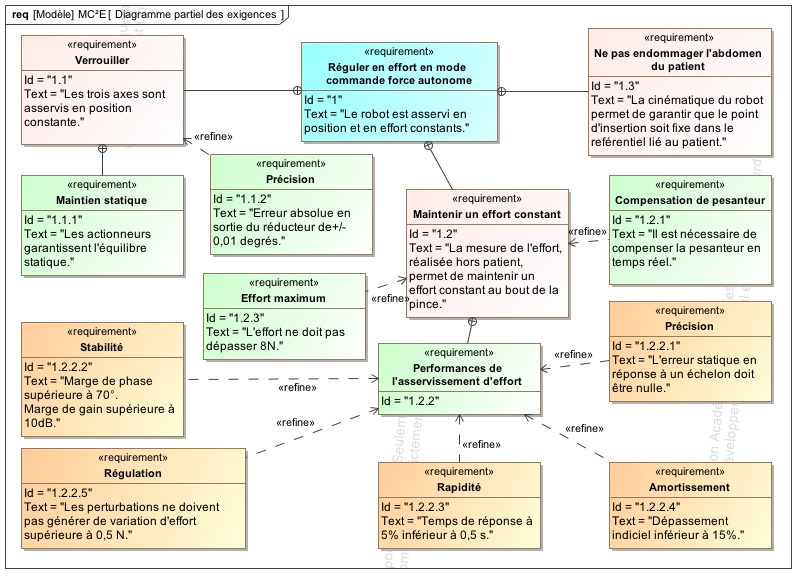
\includegraphics[width=\linewidth]{fig_05}
\caption{Évolutions simulées de $\omega_m(t)$.}
\label{cy_01_ch_02_03_td_03_fig_05}
\end{marginfigure}




\begin{question}
Pour les courbes 1 et 2 de la figure \ref{cy_01_ch_02_03_td_03_fig_05}, préciser, en le justifiant, la simulation qui est associée à la plus grande
valeur de $K_p$. On pourra exprimer le coefficient d'amortissement de la FTBF ou exprimer l'écart statique.
\end{question}
\ifprof
\begin{corrige}
\textbf{Méthode 1 -- Coefficient d'amortissement}

On note $\indice{H}{BF}(p) = \dfrac{\omega_m(t)}{\indice{\omega}{cons}(t)}$.


On a alors, $\indice{H}{BF}(p) = K_c \dfrac{K_p \ordredeux }{1+K_p \ordredeux  K_c}$
$=  \dfrac{K_cK_p K}{1+\dfrac{2\xi}{\omega_0}p+\dfrac{p^2}{\omega_0^2}+K_p K_c}$.

On a donc $\dfrac{2\indice{\xi}{BF}}{\indice{\omega}{BF}} = \dfrac{2\xi}{\omega_0\left(1+K_p K_c\right)}$
et $\indice{\omega}{BF}^2 = \omega_0^2 \left(1+K_p K_c\right)$.

Soit
$\indice{\xi}{BF} = \dfrac{\xi\indice{\omega}{BF}}{\omega_0\left(1+K_p K_c\right)}$ 
$= \dfrac{\xi\omega_0\sqrt{1+K_p K_c}}{\omega_0\left(1+K_p K_c\right)}$ 
$= \dfrac{\xi}{\omega_0\sqrt{1+K_p K_c}}$.

En conclusion, plus $K_p$ augmente, plus le coefficient d'amortissement diminue et donc plus les pseudo oscillations deviennent grandes. La courbe 2 a donc la plus grande valeur de $K_p$.

\textbf{Méthode 2 -- Calcul de l'écart statique}

On montre que $\varepsilon(p) = \indice{\omega}{cons}(p) K_a \dfrac{1}{1+FTBO(p)}$
$= \dfrac{\indice{\omega}{cons}(p) K_a}{1+K_p K_c\ordredeux }$.

Pour une entrée échelon et en utilisant le théorème de la valeur finale, on a 
$\varepsilon_S =  \lim\limits_{t\to +\infty} = \varepsilon(t) = \lim\limits_{p\to 0} p \varepsilon(p)$
$\lim\limits_{p\to 0} \dfrac{ K_a}{1+K_p K_c\ordredeux } = \dfrac{K_a}{1+K_p K_c K}$.

Lorsque $K_p$ augmente, $ \varepsilon_S$ diminue. La courbe 2 a donc la plus grande valeur de $K_p$.



\end{corrige}
\else
\fi

\begin{question}
Pour chaque courbe de la figure \ref{cy_01_ch_02_03_td_03_fig_05}, préciser, en le justifiant, si la valeur de $K_i$ est nulle ou non.
\end{question}
\ifprof
\begin{corrige}
On montre que $\varepsilon(p) = \indice{\omega}{cons}(p) K_a \dfrac{1}{1+FTBO(p)}$
$= \dfrac{\indice{\omega}{cons}(p) K_a}{1+\left( K_p + \dfrac{K_i}{p}\right) K_c\ordredeux }$.

Pour une entrée échelon et en utilisant le théorème de la valeur finale, on a 
$\varepsilon_S =  \lim\limits_{t\to +\infty} = \varepsilon(t) = \lim\limits_{p\to 0} p \varepsilon(p) = 0$.
Ainsi, si $K_i$ non nul, $\varepsilon_S  =0$ (courbe 3 uniquement).

\end{corrige}
\else
\fi




\begin{question}
Déterminer les valeurs associées aux quatre critères de performances de l’exigence 1.2.2.1.
Conclure sur le correcteur à adopter.
\end{question}
\ifprof
\begin{corrige}
\footnotesize
\begin{tabular}{llllll}
\hline 
 & Stabilité & 1\ier Dépassement & Erreur statique & $T_{5\%}$ \\
 \hline 
 Exigences &  Absolue & $< 20\, \%$ & Nulle & $\SI{0,5}{s}$ \\
 Courbe 1 & Stable \textbf{OK} & $D_1 = \SI{45}{\%}$ \textbf{Pas OK} &$\SI{2450}{tr/min} $ \textbf{Pas OK}&$T_{5\%} = \SI{0,015}{s}$ \textbf{ OK}\\
 Courbe 2 & Stable \textbf{OK} & $D_1 = \SI{59}{\%}$ \textbf{Pas OK} &$\SI{900}{tr/min} $ \textbf{Pas OK}&$T_{5\%} = \SI{0,018}{s}$ \textbf{ OK}\\
  Courbe 3 & Stable \textbf{OK} & $D_1 = \SI{15}{\%}$ \textbf{OK} &$\SI{0}{tr/min} $ \textbf{OK}&$T_{5\%} = \SI{0,048}{s}$ \textbf{ OK}\\
 \hline
 \end{tabular}

\normalsize
\end{corrige}
\else
\fi


\ifcolle
\else
\ifprof
\else
\marginnote[-2cm]{
\begin{solution}
\begin{enumerate}[wide, labelwidth=!, labelindent=0pt]
\item .
\item $K_a = K_c$.
\item .
\item $K= \dfrac{1}{k_e}$, $\omega_0 =\sqrt{ \dfrac{k_ck_e}{JL}}$ et
$\xi =  \dfrac{R\sqrt{J}}{2 \sqrt{L k_ck_e}} $.
\item La courbe 2 a la plus grande valeur de $K_p$.
\item $K_i\neq 0 $ pour la courbe 3 uniquemement.
\item .
\end{enumerate}
\end{solution}}
\fi
\fi



\ifprof
\else
\begin{marginfigure}[4.5cm]
\centering
\fancyqr{http://xpessoles-cpge.fr/pdf/Cy_01_Ch_02_03_TD_04_Tissus_Corrige.pdf}
\end{marginfigure}
\fi